\documentclass[technote,a4paper,leqno]{IEEEtran}
\pdfoutput=1

% packages
\usepackage[utf8]{inputenc}
\usepackage[T1]{fontenc}
\usepackage{amsmath,amssymb}
\usepackage[pdftex]{graphicx}
\usepackage{caption}
\usepackage[hang]{subfigure}
\captionsetup{format=hang}
\usepackage{url}
\usepackage[super]{nth}
\usepackage[breaklinks]{hyperref}
\def\UrlBreaks{\do\/\do-}
\usepackage[absolute,overlay]{textpos}
\usepackage{tikz}
\usepackage{csquotes}
\usepackage{booktabs}  % for \toprule, \midrule and \bottomrule
\usepackage{pbox}
\usepackage{braket} % needed for nice printing of sets
\usepackage[english]{babel}
\usepackage{mathtools}
\usepackage{xspace}
\usepackage[inner=2.5cm,outer=2.5cm,top=2.5cm,bottom=2cm,includeheadfoot]{geometry}
\usepackage[xindy,toc]{glossaries}
\loadglsentries[main]{glossary}
\makeglossaries

\usepackage[nameinlink, noabbrev,capitalise]{cleveref} % has to be after hyperref, nthe l.137 ...eam attr{/N 4}  file{sRGBIEC1966-2.1.icmorem, amsthm


% List stuff
\usepackage{enumitem}
\crefname{problemnr}{\textup{problem}}{\textup{problems}}
\newlist{problemnr}{enumerate}{1}
\setlist[problemnr]{label={P\arabic*}, ref=P\arabic*}
\crefalias{problemnri}{problemnr}

\newcommand*{\eg}{e.g.\@\xspace}


\usepackage[binary-units,group-separator={,}]{siunitx}
\sisetup{per-mode=fraction,
         binary-units=true,
         group-separator = {\,},
         range-phrase=-}
\DeclareSIUnit\pixel{px}
\usepackage{microtype}

\DeclareGraphicsExtensions{.jpg}
\DeclareMathOperator{\sgn}{sgn}
\DeclareMathOperator*{\minimize}{minimize}
\DeclareMathOperator*{\maximize}{maximize}

\newcommand\independent{\protect\mathpalette{\protect\independenT}{\perp}}
\def\independenT#1#2{\mathrel{\rlap{$#1#2$}\mkern2mu{#1#2}}}

\newcommand{\titleboth}{A Survey of Semantic Segmentation}
\title{\titleboth}
\author{Martin Thoma\\% ORCID: http://orcid.org/0000-0002-6517-1690 Thoma, Martin
info@martin-thoma.de
}

\hypersetup{
    pdfauthor   = {Martin Thoma},
    pdfkeywords = {semantic segmentation, pixelwise classification, pixel-level classification},
    pdfsubject  = {Segmentation},
    pdftitle    = {\titleboth},
}

\begin{document}
\maketitle
\input{00-abstract.tex}

\input{01-introduction}
%!TEX root = vorlage.tex

\section{Taxonomy of Segmentation Algorithms}\label{sec:taxonomy}
The computer vision community has published a wide range of segmentation
algorithms so far. Those algorithms can be grouped by the kind of data they
operate on and the kind of segmentation they are able to produce.

The following subsections will give four different criteria by which
segmentation algorithms can be classified.

This survey describes fixed-class (see \cref{subsec:allowed-classes}),
single-class affiliation (see \cref{subsec:class-affiliation}) algorithms which
work on grayscale or colored single pixel images (see \cref{subsec:input-data})
in a completely automated, passive fashion (see \cref{subsec:operation-state}).


\subsection{Allowed classes}\label{subsec:allowed-classes}
Semantic segmentation is a classification task. As such, the classes on which
the algorithm is trained is a central design decision.

Most algorithms work with a fixed set of classes; some even only work on binary
classes like \textit{foreground vs
background}~\cite{4228537,carreira2010constrained} or \textit{street vs no
street}~\cite{bittel2015pixel}.

However, there are also unsupervised segmentation algorithms which do not
distinguish classes at all (see
\cref{subsec:unsupervised-traditional-segmentation}) as well as segmentation
algorithms which are able to recognize when they don't know a class. For
example, in~\cite{gould2008multi} a
\textbf{void class} was added for classes which were not in the training set.
Such a void class was also used in the MSRCv2 dataset (see
\cref{subsubsec:MSRCv2}) to make it possible to make more coarse segmentations
and thus having to spend less time annotating the image.


\subsection{Class affiliation of pixels}\label{subsec:class-affiliation}
Humans do an incredible job when looking at the world. For example, when we see
a glass of water standing on a table we can automatically say that there is the
glass and behind it the table, even if we only had a single image and were not
allowed to move. This means we simultaneously two labels to the coordinates of
the glass: Glass and table. Although there is much more work being done on
\textbf{single class affiliation} segmentation algorithms, there is a
publication about \textbf{multiple class affiliation}
segmentation~\cite{levin2008spectral}. Similarly, recent publications in
pixel-level object segmentation used layered models~\cite{yang2012layered}.

\goodbreak
\subsection{Input Data}\label{subsec:input-data}
The available data which can be used for the inference of a segmentation varies
by application.

\begin{itemize}
    \item \textbf{Grayscale vs colored}: Grayscale images are commonly used in
          medical imaging such as \gls{MR} imaging or ultrasonography whereas
          colored photographs are obviously widespread.
    \item \textbf{Excluding or including depth data}: RGB-D, sometimes also
          called range~\cite{hoover1996experimental} is available in robotics,
          autonomous cars and recently also in consumer electronics such as
          Microsoft Kinect~\cite{6190806}.
    \item \textbf{Single image vs stereo images vs co-segmentation}: Single
          image segmentation is the most wide-spread kind of segmentation, but
          using stereo images was already tried in~\cite{boykov2001fast}. It
          can be seen as a more natural way of segmentation as most mammals
          have two eyes. It can also be seen as being related to having
          depth data.\\
          Co-segmentation as in~\cite{1640859,collins2012random} is the problem
          of finding a consistent segmentation for multiple images. This problem
          can be seen in two ways: One the one hand, it can be seen as the problem
          of finding common objects in at least two images. On the other hand,
          every image after the first can be used as an additional source of
          information to find a meaningful segmentation. This idea can be
          extended to time series such as videos.
    \item \textbf{2D vs 3D}: Segmenting images is a 2D~segmentation task where
          the smallest unit is called a \textit{pixel}. In 3D data, such as
          volumetric X-ray CT images as they were used in~\cite{929615}, the
          smallest unit is called a voxel.
\end{itemize}


\subsection{Operation state}\label{subsec:operation-state}
The operation state of the classifying machine can either be \textbf{active} as
in~\cite{schiebener2011segmentation,schiebener2012discovery} where robots can
move objects to find a segmentation or \textbf{passive}, where the received
image cannot be influenced. Among the passive algorithms, some segment in a
completely \textbf{automatic} fashion, others work in an \textbf{interactive}
mode. One example would be a system where the user clicks on the background or
marks a coarse segmentation and the algorithm finds a fine-grained
segmentation.
\cite{boykov2000interactive,rother2004grabcut,protiere2007interactive}~describe
systems which work in an interactive mode.

\input{02-0-evaluation-and-datasets}
%!TEX root = vorlage.tex

\section{Segmentation Pipeline}

Typically, semantic segmentation is done with a classifier which operates on
fixed-size feature inputs and a \textit{sliding-window}
approach~\cite{1467360,5490399,schroff2008object}. This means a classifier is
trained on images of a fixed size. The trained classifier is then fed with
rectangular regions of the image which are called \textit{windows}. Although
the classifier gets an image patch of e.g. $\SI{51}{\pixel} \times
\SI{51}{\pixel}$ of the environment, it classifies only the center pixel. This
segmentation pipeline is visualized in~\cref{fig:segmentation-pipeline}.

\begin{figure}
    \centering
    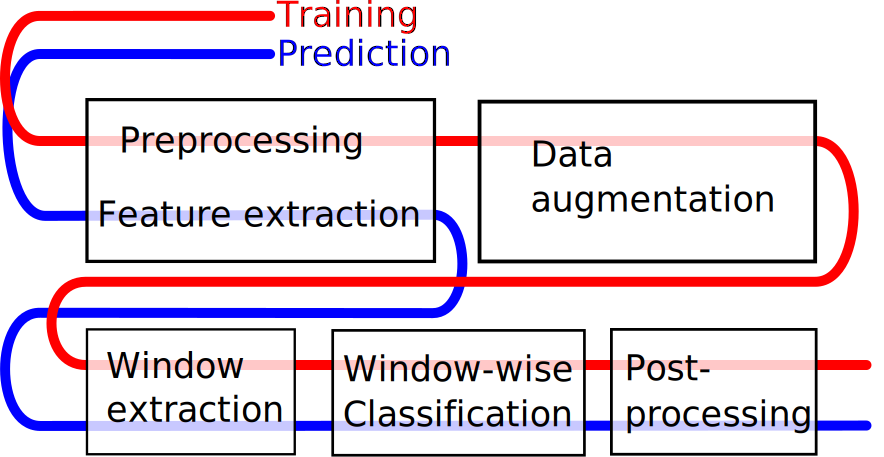
\includegraphics[width=\linewidth, keepaspectratio]{figures/segmentation-pipeline.pdf}
    \caption{A typical segmentation pipeline gets raw pixel data, applies
             preprocessing techniques like scaling and feature extraction like
             HOG features. For training, data augmentation techniques such as
             image rotation can be applied. For every single image, patches
             of the image called \textit{windows} are extracted and those
             windows are classified. The resulting semantic segmentation can
             be refined by simple morphologic operations or by more complex
             approaches such as \glspl{MRF}.}
    \label{fig:segmentation-pipeline}
\end{figure}

This approach was taken by~\cite{bittel2015pixel} and a majority of the VOC2007
participants~\cite{pascal-voc-2007}. As this approach has to apply the patch
classifier $512 \cdot 512 = \num{262144}$ times for images of size
$\SI{512}{\pixel} \times \SI{512}{\pixel}$, there are techniques for speeding
it up such as applying a stride and interpolating the results.

Neural networks are able to apply the sliding window approach in a very
efficient way by handling a trained network as a convolution and applying the
convolution on the complete image.

However, there are alternatives. Namely \glspl{MRF} and \glspl{CRF}
which take the information of the complete image and segment it in an holistic
approach.

%!TEX root = vorlage.tex

\section{Traditional Approaches}\label{sec:traditional-approaches}%
Image segmentation algorithms which use traditional approaches, hence don't
apply neural networks and make heavy use of domain knowledge, are wide-spread
in the computer vision community. Features which can be used for segmentation
are described in \cref{subsec:features}, a very brief overview of unsupervised,
non-semantic segmentation is given in
\cref{subsec:unsupervised-traditional-segmentation}, Random Decision
Forests are described in \cref{subsec:random-forests}, Markov Random Fields in \cref{subsec:markov-random-fields}
 and \glspl{SVM} in
\cref{subsec:trad-SVM}.
Postprocessing is covered in \cref{subsec:post-processing-methods}.

It should be noted that algorithms can use combination of methods. For example,
\cite{tighe2014scene} makes use of a combination of a \gls{SVM} and a
\gls{MRF}. Also, auto-encoders can be used to learn features which in turn
can be used by any classifier.

\input{03-2-features}
\input{03-3-unsupervised}
\input{03-4-random-forests}
\input{03-traditional-svm}
%!TEX root = vorlage.tex

\subsection{Markov Random Fields}\label{subsec:markov-random-fields}
\tikzstyle{pixel}=[draw,black,circle,minimum size=10pt,inner sep=0pt,fill=red!50]
\tikzstyle{label}=[draw,black,circle,minimum size=10pt,inner sep=0pt,fill=blue!50]
\tikzstyle{edge}=[very thick]
\begin{figure}
    \centering
\begin{tikzpicture}[scale=1.7]
    \node (x1)[pixel] at (0.0,1.15) {$x_1$};
    \node (x2)[pixel] at (1.0,1.15) {$x_2$};
    \node (x3)[pixel] at (2.0,1.15) {$x_3$};
    \node (x4)[pixel] at (0.5,1.65) {$x_4$};
    \node (x5)[pixel] at (1.5,1.65) {$x_5$};
    \node (x6)[pixel] at (2.5,1.65) {$x_6$};
    \node (x7)[pixel] at (1.0,2.15) {$x_7$};
    \node (x8)[pixel] at (2.0,2.15) {$x_8$};
    \node (x9)[pixel] at (3.0,2.15) {$x_9$};

    \node (y1)[label] at (0.0,1.5) {$y_1$};
    \node (y2)[label] at (1.0,1.5) {$y_2$};
    \node (y3)[label] at (2.0,1.5) {$y_3$};
    \node (y4)[label] at (0.5,2.0) {$y_4$};
    \node (y5)[label] at (1.5,2.0) {$y_5$};
    \node (y6)[label] at (2.5,2.0) {$y_6$};
    \node (y7)[label] at (1.0,2.5) {$y_7$};
    \node (y8)[label] at (2.0,2.5) {$y_8$};
    \node (y9)[label] at (3.0,2.5) {$y_9$};

    \draw[edge] (y1) -- (y2);
    \draw[edge] (y1) -- (y4);
    \draw[edge] (y2) -- (y3);
    \draw[edge] (y2) -- (y5);
    \draw[edge] (y3) -- (y6);
    \draw[edge] (y4) -- (y5);
    \draw[edge] (y4) -- (y7);
    \draw[edge] (y5) -- (y6);
    \draw[edge] (y5) -- (y8);
    \draw[edge] (y6) -- (y9);
    \draw[edge] (y7) -- (y8);
    \draw[edge] (y8) -- (y9);

    \draw[edge] (x1) -- (y1);
    \draw[edge] (x2) -- (y2);
    \draw[edge] (x3) -- (y3);
    \draw[edge] (x4) -- (y4);
    \draw[edge] (x5) -- (y5);
    \draw[edge] (x6) -- (y6);
    \draw[edge] (x7) -- (y7);
    \draw[edge] (x8) -- (y8);
    \draw[edge] (x9) -- (y9);

    %\draw [dashed] (-0.5,-0.3) -- (2,-0.3) -- (3.5,1.5) -- (0.5,1.5) -- (-0.5,-0.3);
    \node (x1)[pixel] at (0.0,1.15) {$x_1$};
    \node (x2)[pixel] at (1.0,1.15) {$x_2$};
    \node (x3)[pixel] at (2.0,1.15) {$x_3$};
    \node (x4)[pixel] at (0.5,1.65) {$x_4$};
    \node (x5)[pixel] at (1.5,1.65) {$x_5$};
    \node (x6)[pixel] at (2.5,1.65) {$x_6$};
    \node (x7)[pixel] at (1.0,2.15) {$x_7$};
    \node (x8)[pixel] at (2.0,2.15) {$x_8$};
    \node (x9)[pixel] at (3.0,2.15) {$x_9$};

    \node (y1)[label] at (0.0,1.5) {$y_1$};
    \node (y2)[label] at (1.0,1.5) {$y_2$};
    \node (y3)[label] at (2.0,1.5) {$y_3$};
    \node (y4)[label] at (0.5,2.0) {$y_4$};
    \node (y5)[label] at (1.5,2.0) {$y_5$};
    \node (y6)[label] at (2.5,2.0) {$y_6$};
    \node (y7)[label] at (1.0,2.5) {$y_7$};
    \node (y8)[label] at (2.0,2.5) {$y_8$};
    \node (y9)[label] at (3.0,2.5) {$y_9$};
\end{tikzpicture}
\caption{\gls{CRF} with 4-neighborhood. Each node $x_i$ represents a pixel and
         each node $y_i$ represents a label.}
\label{fig:crf-image}
\end{figure}
\Glspl{MRF} are undirected probabilistic graphical models which are wide-spread
model in computer vision. The overall idea of \glspl{MRF} is to assign a random
variable for each feature and a random variable for each pixel which gets
labeled as shown in~\cref{fig:crf-image}. For example, a \gls{MRF} which is
trained on images of the size
$\SI{224}{\pixel} \times \SI{224}{pixel}$ and gets the raw RGB values as
features has
\[\underbrace{224 \cdot 224 \cdot 3}_{\text{input}} + \underbrace{224 \cdot 224}_{\text{output}} = \num{200704}\]
random variables. Those random variables are conditionally independent, given
their local neighborhood. These (in)dependencies can be expressed with a graph.

Let $G=(\mathcal{V}, \mathcal{E})$ be the associated undirected graph of an
\gls{MRF} and $\mathcal{C}$ be the set of all maximal cliques in that graph.
Nodes represent random variables $\mathbf{x}, \mathbf{y}$ and edges represent
conditional dependencies. Just like in
\crefname{subsec:graph-based-image-segmentation}, the
4-neighborhood~\cite{shotton2006textonboost} and the 8-neighborhood are
reasonable choices for constructing the graph.

Typically, random variables $\mathbf{y}$ represent the class of a single pixel,
random variables $\mathbf{x}$ represent a pixel values and edges represent
pixel neighborhood in computer vision problems segmentation problems where
\glspl{MRF} are used. Accordingly, the random variables $\mathbf{y}$ live on
$1, \dots, \text{nr of classes}$ and the random variables $\mathbf{x}$
typically live on $0, \dots, 255$ or $[0, 1]$.

The probability of $\mathbf{x}, \mathbf{y}$ can be expressed as
\[P(\mathbf{x}, \mathbf{y}) = \frac{1}{Z} e^{-E(\mathbf{x}, \mathbf{y})}\]
where $Z = \sum_{\mathbf{x}, \mathbf{y}} e^{-E(\mathbf{x}, \mathbf{y})}$ is a normalization term called
the \textit{partition function} and $E$ is called the \textit{energy function}.
A common choice for the energy function is
\[E(\mathbf{x}, \mathbf{y}) = \sum_{c \in \mathcal{C}} \psi_c(\mathbf{x}, \mathbf{y})\]
where $\psi$ is called a \textit{clique potential}. One choice for cliques
of size two $\mathbf{x}, \mathbf{y} = (x_1, x_2)$ is~\cite{kato2006markov}
\[\psi_c(x_1, x_2) = w \delta(x_1, x_2) = \begin{cases}+w &\text{if } x_1 \neq x_2\\-w &\text{if } x_1 = x_2\end{cases}\]

According to~\cite{murphy2012machine}, the most common way of inference over
the posterior \gls{MRF} in computer vision problems is \gls{MAP} estimation.


Detailed introductions to \glspl{MRF} are given by
\cite{blake2011markov,murphy2012machine}. \glspl{MRF} are used by \cite{zhang2001segmentation} and \cite{moser2012markov}
for image segmentation.

% Characterizations of MRF:
% Label space: binary vs multi-label; homogeneous vs heterogeneous
% Order: unary vs pairwise vs higher-order
% Structure: chain vs tree vs grid vs general graph; neighborhood size
% Potentials: submodular, convex, compressible

% Markov Random Fields for Computer Vision (Part 1)
% http://users.cecs.anu.edu.au/~sgould/papers/part1-MLSS-2011.pdf  --- very nice!
% http://users.cecs.anu.edu.au/~sgould/papers/part2-MLSS-2011.pdf
% http://users.cecs.anu.edu.au/~sgould/papers/part3-MLSS-2011.pdf

% Markov Random Field Image Models and Their Applications to Computer Vision
% http://www.mathunion.org/ICM/ICM1986.2/Main/icm1986.2.1496.1517.ocr.pdf


\subsection{Conditional Random Fields}\label{subsec:conditional-random-fields}

\Glspl{CRF} are \glspl{MRF} where all clique potentials are conditioned on
input features~\cite{murphy2012machine}. This means, instead of learning the
distribution $P(\mathbf{y}, \mathbf{x})$, the task is reformulated to learn the
distribution $P(\mathbf{y}| \mathbf{x})$. One consequence of this reformulation
is that \glspl{CRF} need much less parameters as the distribution of
$\mathbf{x}$ does not have to be estimated. Another advantage of \glspl{CRF}
compared to \glspl{MRF} is that no distribution assumption about $\mathbf{x}$
has to be made.

A \gls{CRF} has the partition function $Z$:
\[Z(\mathbf{x}) = \sum_{\mathbf{y}} P(\mathbf{x}, \mathbf{y})\]

and joint probability distribution

\[P(\mathbf{y} | \mathbf{x}) = \frac{1}{Z(\mathbf{x})} \prod_{c \in \mathcal{C}} \psi_c(\mathbf{y}_c | \mathbf{x})\]

The simplest way to define the clique potentials $\psi$ is the count of the
class $\mathbf{y}_c$ given $\mathbf{x}$ added with a positive smoothing
constant to prevent the complete term from getting zero.

\Glspl{CRF} as described in~\cite{associative09} have reached top performance
in PASCAL VOC 2010~\cite{VOC2010Results} and are also used in
\cite{multiscale04,shotton2006textonboost} for semantic segmentation.

A method similar to \glspl{CRF} was proposed in~\cite{gonfaus2010harmony}.
The system of Gonfaus~et.al. ranked~\nth{1} by mean accuracy in the segmentation
task of the PASCAL VOC 2010 challenge~\cite{everingham2010pascal}.

An introduction to \glspl{CRF} is given by~\cite{sutton2011introduction}.

\input{03-traditional-post-processing}

\input{04-nn-approaches}
\input{05-typical-problems}
\input{06-discussion}

\newpage
\bibliography{literature}
\bibliographystyle{IEEEtranSA}\vfill
% \columnbreak
\printglossaries%

\input{appendix}

\end{document}
